\documentclass{beamer}
\usepackage{amssymb}
\usepackage{amsmath}
\usepackage{commath}
\usepackage{amsthm}
\usepackage{lmodern}
\usepackage{scrextend}
\usepackage{stmaryrd}
\usepackage{xcolor}
\definecolor{mediumred-violet}{rgb}{0.73, 0.2, 0.52}
\definecolor{jasper}{rgb}{0.84, 0.23, 0.24}
\usepackage{capt-of}
\usepackage{tikz}
\newcommand*\diff{\mathop{}\!\mathrm{d}}
\usetheme{Frankfurt}
\useoutertheme[subsection=false, footline=authortitle]{miniframes}
\usecolortheme{seagull}
\newtheorem{prop}{Proposition}

\title{The polluted atmosphere as a shallow domain}
\author[N\'ora Juh\'asz] { \textbf{N\'ora Juh\'asz} \\[1mm] \textit{Collaborators: Prof. Donatella Donatelli, Prof. Omar Lakkis}}
\vspace{10mm}
\institute{Department of Information Engineering, Computer Science and Mathematics \\ University of L'Aquila }

\date{5th June, 2020}

\logo{
    
\includegraphics[width=1cm,height=1cm,keepaspectratio]{LogoModCompShock.jpg}\hspace*{10.5cm}~%
    
\includegraphics[width=1cm,height=1cm,keepaspectratio]{LogoDisim.png}~%
}

\begin{document}

\begin{frame}
\titlepage
\end{frame}

%%% MODELLING FOUNDATIONS %%%
\section{Modelling foundations}

\begin{frame}{Conservation laws of geophysical fluids}

\textbf{Starting point:} a comprehensive picture of the relationship between the variables in atmosphere modelling.

$$ \partial_t \rho + \nabla \cdot (\rho \mathbf{v})  = 0 \quad \text{ in } \Omega_0 \times (0,T), $$

$$ \partial_t (\rho \mathbf{v}) + \rho (\mathbf{v} \cdot \nabla)\mathbf{v} -\Delta_{\nu} \mathbf{v} + \nabla q = \rho \mathbf{g} \quad \text{ in } \Omega_0 \times (0,T), $$

$$ \partial_t \tau + \mathbf{v} \nabla \tau = k \Delta \tau + \frac{Q}{\rho C_\rho} \quad \text{ in } \Omega_0 \times (0,T), $$

$$ \rho = f(\tau, q)  \quad \text{ in } \Omega_0 \times (0,T). $$

\end{frame}

\begin{frame}{Four basic concepts we use}

We combine these equations with the following four basic concepts.

\begin{enumerate}

\item \textbf{The Coriolis force}: $2 \omega \times \mathbf{v}$ --- due to working with a large-scale phenomena on the surface of the rotating Earth.
\item \textbf{The Boussinesq approximation}: a simplification used in so-called Boussinesq flows (atmospheric fronts, oceanic circulation, natural ventilation) is to use $\rho \equiv \rho_0$ everywhere except in the gravity term and the state equation.
\item The notion of an \textbf{isothermal process}: $\tau \equiv \tau_0,$ and as a consequence, $\rho \equiv \rho_0$ everywhere.
\item \textbf{The incompressibility condition}: a consequence of the Boussinesq approximation.

\end{enumerate}

\end{frame}

\begin{frame}{Incompressible Navier-Stokes equations}

Incorporating these ideas we arrive to the incompressible Navier-Stokes equations:

$$ \partial_t \mathbf{v} + (\mathbf{v} \cdot \nabla)\mathbf{v} -\Delta_{\nu} \mathbf{v} + \nabla q + 2 \mathbf{\omega} \times \mathbf{v}= \mathbf{g} \text{ in } \Omega_0 \times (0,T), $$
    
$$ \nabla \cdot \mathbf{v} = 0 \text{ in } \Omega_0 \times (0,T). $$

\textit{Important}: in all three space dimensions we have a \textbf{complete momentum equation} for the velocity.

\end{frame}

\begin{frame}{Hydrostatic Approximation}

\textbf{Point of apparent theoretical conflict:} The previously described model is \textbf{not} what is widely used in meteorology and oceanology to describe geophysical processes.

The fundamental equations in meteorology -- \textbf{primitive equations}.

$$ \partial_t \mathbf{v}_h + \mathbf{v}_h \cdot \nabla_h \mathbf{v}_h + v_3 \partial_z \mathbf{v}_h - \Delta_{\nu} \mathbf{v}_h + \nabla_h q + 2 (\mathbf{\omega} \times \mathbf{v})_h = 0, $$

$$ \frac{\partial q}{\partial z} = - \mathbf{g}, $$

$$ \nabla \cdot \mathbf{v} = 0. $$

\begin{center}
\textit{Experience shows:} This natural simplification is highly

accurate for large-scale fluids. 
\end{center}

\end{frame}

\begin{frame}

\textbf{A natural question to ask:} 

\begin{enumerate}
  \item Is this valid?
  \item What makes it valid?
\end{enumerate}

\textbf{Justification:} An analytical proof.

\setbeamertemplate{itemize items}[circle]
\begin{itemize}

  \item Key: \textbf{\textit{"we are considering a large-scale geophysical fluid on the surface of the Earth"}} $\to$ mathematical terms.

  \item Scale analysis will show that the dominant term in the full vertical momentum equation is $\frac{\partial q}{\partial z}$ and the gravity term, resulting in the hydrostatic approximation.

\end{itemize}

\end{frame}

\begin{frame}{Adding a contaminant to the system}

We extend the velocity system:
\begin{center}
\textcolor{mediumred-violet}{pollutant present in the atmosphere in concentration $p_c.$}
\end{center}

\textit{The two most important concepts are}

\begin{enumerate}
\item \textbf{diffusion}: molecules move from a region of high concentration to a region of lower concentration,
\item \textbf{convection}: the contaminant is transported by the wind.
\end{enumerate}

The movement of pollutants is modelled by the continuity equation

$$\partial_t p_c + \mathbf{v} \cdot \nabla p_c = \nabla \cdot (\mathbf{K} \nabla p_c) + q_c \quad \text{ in } \Omega_0 \times (0,T). $$

\end{frame}

\begin{frame}{Scaling - shallowness part 1}

\textbf{"$\beta$-plane approximation"} $\to$ this means that we can neglect the curvature of the Earth (valid locally) $\to$ we can use Cartesian coordinates.

Geophysical fluid: shallow domain characteristics --- the domain is greater horizontally than in the vertical dimension.

$$\textcolor{jasper}{\epsilon} = \frac{\text{characteristic depth}}{\text{characteristic width}} = \text{aspect ratio}.$$

\textbf{Natural scaling process:}

$$ x=x_1, y=x_2, z= \textcolor{jasper}{\epsilon} x_3,$$
$$ v_1 = u_1^{\epsilon}, v_2 = u_2^{\epsilon}, v_3 = \textcolor{jasper}{\epsilon} u_3^{\epsilon}, p = p^{\epsilon}, $$
$$ p_c = \frac{1}{\textcolor{jasper}{\epsilon}} c^\epsilon, q_c = \frac{1}{\textcolor{jasper}{\epsilon}} s^\epsilon. $$

\end{frame}

\begin{frame}{Scaling - shallowness part 2}
We need to consider the highly anisotropic nature of viscosity and diffusivity $\to$ this means that these rates are strongly different in horizontal and vertical directions.
Rescaling these parameters according to the largely different scales:


$$ \nu_x = \nu_1, \quad \nu_y = \nu_2 , \quad \nu_z = \textcolor{jasper}{\epsilon^2} \nu_3, $$

\begin{gather}
      \begin{bmatrix} K_{xx} & K_{xy} & K_{xz} \\ K_{yx} & K_{yy} & K_{yz} \\ K_{zx} & K_{zy} & K_{zz} \end{bmatrix}
       =
      \begin{bmatrix}
    M_{11} & M_{12} & \textcolor{jasper}{\epsilon} M_{13} \\ M_{21} & M_{22} & \textcolor{jasper}{\epsilon} M_{23} \\ \textcolor{jasper}{\epsilon} M_{31} & \textcolor{jasper}{\epsilon} M_{32} & \textcolor{jasper}{\epsilon^2} M_{33}
  \end{bmatrix}. \nonumber
\end{gather}

  
The diffusivity matrix is assumed to be coercive: $\lambda \norm{\mathbf{x}}^2 \leq (\mathbf{M} \mathbf{x}, \mathbf{x}).$

\end{frame}

\begin{frame}{Source term}

We consider a contaminant plume
\begin{itemize}
\item with intensity $I,$
\item originating at emission coordinates $\mathbf{x}_s,$
\item beginning at time $t_s.$
\end{itemize}

We arrive to the complete source term model of the form
%
$$s_\eta (t, t_s, x, x_s) = I H(t-t_s) \delta_\eta (\mathbf{x} - \mathbf{x}_s), $$
%
where $\delta_\eta$ is an approximated delta function.

\end{frame}

\begin{frame}{Source term part 2}
We reformulate the above expression in terms of $\textcolor{jasper}{\epsilon}$ --- new parameter of the distribution.

The following function will give shape to the source term:
%
$$
\delta_\epsilon (\mathbf{x}) = 
  \begin{cases}
       \frac{1}{\textcolor{jasper}{\epsilon^3}} \exp{\bigg ( \frac{1}{\abs{{\frac{\mathbf{x}}{\textcolor{jasper}{\epsilon}}}}^2-1} \bigg ) } &\quad \abs{\mathbf{x}} < \textcolor{jasper}{\epsilon} \\
       0 &\quad \abs{\mathbf{x}} \geq \textcolor{jasper}{\epsilon}, \\
  \end{cases}
$$
%
and finally

$$s^\epsilon = I H(t-t_s) \delta_\epsilon (\mathbf{x} - \mathbf{x}_s).$$
\end{frame}

%%% GFC %%%
\section{Geophysical coordinates}

\begin{frame}{Geophysical coordinates}

$x$ --- East, $y$ --- North, $z$ --- Vertical coordinate (zenith).

\textbf{Result: simpler Coriolis term.}

Earth rotation angular speed: $\omega = f (0, \cos(l(x_2)), \sin(l(x_2))).$ 

The Coriolis acceleration becomes

\begin{gather} \nonumber
2 \omega \times \mathbf{v}
=
\begin{bmatrix} 0 \\ \beta \\ \alpha \end{bmatrix}
 \times
 \begin{bmatrix} u^\epsilon_1 \\ u^\epsilon_2 \\ \textcolor{jasper}{\epsilon} u^\epsilon_3 \end{bmatrix}
 =
 \begin{bmatrix}  \beta \textcolor{jasper}{\epsilon} u^\epsilon_3 - \alpha u^\epsilon_2 \\ \alpha u^\epsilon_1  \\ - \beta u^\epsilon_1 \end{bmatrix},
\end{gather}

where we use $\alpha = 2f \sin(l(x_2)), \beta = 2f \cos(l(x_2)).$

\end{frame}

\begin{frame}{Anisotropic equations}

$$ \partial_t u^\epsilon _1 + \mathbf{u}^\epsilon \cdot \nabla u^\epsilon _1 -\Delta_\nu u^\epsilon _1 -\alpha u_2^\epsilon + \textcolor{jasper}{\epsilon} \beta u_3^\epsilon + \partial_1 p^\epsilon = 0 \text{ in } \Omega \times (0,T) $$

$$ \partial_t u_2^\epsilon + \mathbf{u}^\epsilon \cdot \nabla u_2^\epsilon -\Delta_\nu u_2^\epsilon + \alpha u_1^\epsilon + \partial_2 p^\epsilon = 0 \text{ in } \Omega \times (0,T) $$

$$ \textcolor{jasper}{\epsilon^2} \{  \partial_t u_3^\epsilon + \mathbf{u}^\epsilon \cdot \nabla u_3^\epsilon -\Delta_\nu u_3^{\epsilon} \} - \textcolor{jasper}{\epsilon} \beta u_1^\epsilon + \partial_3 p^\epsilon = 0 \text{ in } \Omega \times (0,T) $$

$$ \nabla \cdot \mathbf{u}^\epsilon= 0 \text{ in } \Omega \times (0,T) $$

$$ \partial_t c^\epsilon + \mathbf{u^\epsilon} \cdot \nabla c^\epsilon = \nabla \cdot (\mathbf{M} \nabla c^\epsilon) + s^\epsilon \text{ in } \Omega \times (0,T) $$

\end{frame}

\begin{frame}{Local domain and boundary conditions}
  \begin{figure}
    
\includegraphics[width=\linewidth]{domain.jpg}
    \caption{A local slice of the atmosphere}
    \label{fig:atmosphere}
  \end{figure}
\end{frame}

\begin{frame}{Anisotropic equations - Part 2}

The initial and boundary conditions are chosen to be
  
\begin{equation} \nonumber \mathbf{u}^\epsilon (\cdot, t = 0) = \mathbf{u}_0, \quad c^\epsilon (\cdot, t=0) = c_0  \quad \text{ in } \Omega, \end{equation}

\begin{equation} \nonumber \mathbf{u}^\epsilon_h = 0, u^\epsilon_3 = 0, c^\epsilon = 0 \text{ on } \Gamma_A \times (0,T), \end{equation}

\begin{equation} \nonumber \nu_3 \partial_3 \mathbf{u}^\epsilon_h = \theta_h, u^\epsilon_3 = 0 \text{ on } \Gamma_G \times (0,T), \end{equation}

\begin{equation} \nonumber \mathbf{M} \nabla c^\epsilon \cdot \vec{\boldsymbol{n}}_{\Gamma_G} = 0 \text{ on } \Gamma_G \times (0,T). \end{equation}

\end{frame}

\begin{frame}{Anisotropic equations}

$$ \partial_t u^\epsilon _1 + \mathbf{u}^\epsilon \cdot \nabla u^\epsilon _1 -\Delta_\nu u^\epsilon _1 -\alpha u_2^\epsilon + \textcolor{jasper}{\epsilon} \beta u_3^\epsilon + \partial_1 p^\epsilon = 0 \text{ in } \Omega \times (0,T) $$

$$ \partial_t u_2^\epsilon + \mathbf{u}^\epsilon \cdot \nabla u_2^\epsilon -\Delta_\nu u_2^\epsilon + \alpha u_1^\epsilon + \partial_2 p^\epsilon = 0 \text{ in } \Omega \times (0,T) $$

$$ \textcolor{jasper}{\epsilon^2} \{  \partial_t u_3^\epsilon + \mathbf{u}^\epsilon \cdot \nabla u_3^\epsilon -\Delta_\nu u_3^{\epsilon} \} - \textcolor{jasper}{\epsilon} \beta u_1^\epsilon + \partial_3 p^\epsilon = 0 \text{ in } \Omega \times (0,T) $$

$$ \nabla \cdot \mathbf{u}^\epsilon= 0 \text{ in } \Omega \times (0,T) $$

$$ \partial_t c^\epsilon + \mathbf{u^\epsilon} \cdot \nabla c^\epsilon = \nabla \cdot (\mathbf{M} \nabla c^\epsilon) + s^\epsilon \text{ in } \Omega \times (0,T) $$

\end{frame}

\begin{frame}{Hydrostatic equations}

$$\partial_t u_1 + \mathbf{u} \cdot \nabla u_1 - \Delta_\nu u_1 - \alpha u_2 + \partial_1 p = 0 \text{ in } \Omega \times (0,T) $$

$$ \partial_t u_2 + \mathbf{u} \cdot \nabla u_2 - \Delta_\nu u_2 + \alpha u_1 + \partial_2 p = 0 \text{ in } \Omega \times (0,T) $$

$$ \partial_3 p = 0 \text{ in } \Omega \times (0,T) $$

$$ \nabla \cdot \mathbf{u} = 0 \text{ in } \Omega \times (0,T) $$

$$ \partial_t c + \mathbf{u} \cdot \nabla c = \nabla \cdot (\mathbf{M} \nabla c) + s \text{ in } \Omega \times (0,T) $$

Initial and boundary conditions are analogous except for using $$ u_1 = u_2 = u_3 n_3 = 0 \text{ on } \Gamma \times (0,T). $$
\end{frame}

\begin{frame}{Fundamental spaces}
\[ C^{\infty}_{\Gamma_A} (\Omega) = \{ \varphi \in C^\infty (\bar{\Omega}); \varphi = 0 \text{ on some neighbourhood of } \Gamma_A \} \]

\[ H^k_{\Gamma_A} (\Omega) = \overline{C_{\Gamma_A} ^ \infty (\Omega)} ^ {H^k (\Omega)} = \{ v \in H^k(\Omega); \partial^\alpha v=0 \text{ on } \Gamma_A \text{ } \forall \alpha \in \mathbb{N}_{k-1} \} \]

\[ \mathbf{V} = \{ \mathbf{v} \in  H^1_{\Gamma_A} (\Omega) \times H^1_{\Gamma_A} (\Omega) \times H^1_0 (\Omega); \nabla \cdot \mathbf{v} = 0 \text{ in } \Omega \} \]

\[ H (\partial_3, \Omega) = \{ v \in L^2(\Omega); \partial_3 v \in L^2 (\Omega)\} \]

\[ H_0 (\partial_3, \Omega) = \overline{C_0 ^\infty (\Omega)}^{H (\partial_3, \Omega)} = \{ v \in H(\partial_3, \Omega); v n_3 = 0 \text{ on } \Gamma \} \]

\[ \mathbf{W} = \{ \mathbf{v} \in  H^1_{\Gamma_A} (\Omega) \times H^1_{\Gamma_A} (\Omega) \times H_0 (\partial_3, \Omega); \nabla \cdot \mathbf{v} = 0 \text{ in } \Omega \} \]
\end{frame}

\begin{frame}{Weak formulation - anisotropic system, part 1}

The pair $(\mathbf{u}^\epsilon, c^\epsilon)$ is a weak solution of the anisotropic system if
$$\mathbf{u}^\epsilon = (\mathbf{u}^\epsilon_h, u^\epsilon_3) \in L^2 (0,T ; \mathbf{V}) \cap L^\infty (0, T; L^2 (\Omega)^3)$$
and
$$c^\epsilon \in L^\infty (0,T; L^2(\Omega)) \cap L^2 (0,T; H^1_{\Gamma_A}(\Omega)),$$ and the following integral identities hold:
%
\begin{equation} \nonumber
\begin{split}
& \int_0^T \bigg [ -(\mathbf{u}^\epsilon_h, \partial_t \mathbf{\tilde{u}}_h) + (\nabla_\nu \mathbf{u}^\epsilon_h, \nabla_\nu \mathbf{\tilde{u}}_h) - (\mathbf{u}^\epsilon_h, (\mathbf{u}^\epsilon \cdot \nabla) \mathbf{\tilde{u}}_h) + (b(\mathbf{u}^\epsilon_h), \mathbf{\tilde{u}}_h) \bigg ] \diff t \\
& + \textcolor{jasper}{\epsilon} \int_0 ^ T \big [ (\beta u_3 ^\epsilon, \tilde{u}_1) - (\beta u_1^\epsilon, \tilde{u}_3) \big ] \diff t\\
& + \textcolor{jasper}{\epsilon^2} \int _0 ^ T \big [ -(u_3^\epsilon, \partial_t \tilde{u}_3) +(\mathbf{u}^\epsilon \cdot \nabla u_3 ^ \epsilon, \tilde{u}_3) + (\nabla_\nu u_3^\epsilon, \nabla_\nu \tilde{u}_3) \big ] \diff t \\
& \hspace{0.3cm} = ({\mathbf{u}_h}_0, \mathbf{\tilde{u}}_h(0)) + \textcolor{jasper}{\epsilon^2} (u_{03}^\epsilon, \tilde{u}_3 (0)) - \int_0^T \langle \theta_h, \mathbf{\tilde{u}}_h \rangle_{\Gamma_G} \diff t
\end{split}
\end{equation}

\end{frame}

\begin{frame}{Weak formulation - anisotropic system, part 2}
 ... and
%
\begin{equation} \nonumber
\begin{split}
& \int_0^T \bigg [ -(c^\epsilon, \partial_t \tilde{c}) -(\mathbf{u}^\epsilon c^\epsilon, \nabla \tilde{c}) + (\mathbf{M} \nabla c^\epsilon, \nabla \tilde{c}) \bigg ] \diff t \\
& =  (c_0, \tilde{c} (0)) + \int_0^T (s^\epsilon,\tilde{c}) \diff t
\end{split}
\end{equation}
%
for all
$$\mathbf{\tilde{u}} = (\mathbf{\tilde{u}}_h, \tilde{u}_3) \in H^1 (0,T;\mathbf{V}) \text{ with } \mathbf{\tilde{u}}(T) = 0$$ and $$\tilde{c} \in H^1 (0,T, H^2_{\Gamma_A} (\Omega)) \text{ with }\tilde{c} (T) = 0.$$
\end{frame}

\begin{frame}{Weak formulation - hydrostatic system, part 1}

The pair $(\mathbf{u}, c)$ is a weak solution of the a hydrostatic system if
$$\mathbf{u} = (\mathbf{u}_h, u_3) \in L^2 (0, T; \mathbf{W}) \text{ with } \mathbf{u}_h \in L^\infty (0,T; L^2(\Omega)^2),$$
and
$$c \in L^\infty(0,T; L^2(\Omega)) \cap L^2(0,T; H^1_{\Gamma_A}(\Omega)),$$ and the following integral identities hold:
%
\begin{equation} \nonumber
\begin{split}
& \int_0^T \bigg[ -(\mathbf{u}_h, \partial_t \mathbf{\tilde{u}}_h) + (\nabla_\nu \mathbf{u}_h, \nabla_\nu \mathbf{\tilde{u}}_h) - (\mathbf{u}_h, (\mathbf{u} \cdot \nabla) \mathbf{\tilde{u}}_h) + (b(\mathbf{u}_h), \mathbf{\tilde{u}}_h) \bigg ] \diff t \\
& = ({\mathbf{u}_h}_0, \mathbf{\tilde{u}}_h(0)) - \int_0^T \langle \theta_h, \mathbf{\tilde{u}}_h \rangle_{\Gamma_G} \diff t
\end{split}
\end{equation}
%
\end{frame}

\begin{frame}{Weak formulation - hydrostatic system, part 2}
... and
%
\begin{equation} \nonumber
\int_0^T \bigg[ -(c, \partial_t \tilde{c}) -(\mathbf{u}c, \nabla \tilde{c}) +  (\mathbf{M} \nabla c, \nabla \tilde{c}) \bigg ] \diff t = (c_0, \tilde{c}(0)) + \int_0^T (s,\tilde{c}) \diff t
\end{equation}
%
for all
$$\mathbf{\tilde{u}} = (\mathbf{\tilde{u}}_h, \tilde{u}_3) \in H^1 (0,T, \mathbf{W}), \mathbf{\tilde{u}}_h (T) = 0 \text{ and } \partial_3 \mathbf{\tilde{u}}_h \in L^\infty (0, T; L^3 (\Omega)^2)$$
and
$$\tilde{c} \in H^1 (0,T, H^2_{\Gamma_A} (\Omega)), \tilde{c} (T) = 0.$$

\end{frame}

\begin{frame}{Main theorem}

We show a rigorous connection between the two sets --- taking the limit in the solutions we arrive to a justification of the hydrostatic model for the case of the polluted atmosphere.

\begin{theorem}
Let $\mathbf{u}_0 \in L^2 (\Omega)$, with $\nabla \cdot \mathbf{u}_0 = 0, \mathbf{u}_0 \cdot \mathbf{n} = 0$ on $\partial \Omega$; $\theta_h \in L^2(0,T; H^{-1/2}(\Gamma_G)),$ let $c_0 \in L^2 (\Omega)$; then as the aspect ratio $\textcolor{jasper}{\epsilon}$ tends to zero, any weak solution $(\mathbf{u}^\epsilon, \textcolor{mediumred-violet}{c^\epsilon})$ of the anisotropic equations converges (up to a subsequence) weakly to a weak solution $(\mathbf{u}, \textcolor{mediumred-violet}{c})$ of the hydrostatic equations of the polluted atmosphere.
\end{theorem}

\changefontsizes{10pt}
\hspace{3mm} To appear in \textit{Mathematical Methods in the Applied Sciences}.

\vspace{2mm}
\hspace{3mm} For details see \textit{D. Donatelli, N. Juhasz, Weak solution of the merged}

\hspace{3mm} \textit{mathematical equations of the polluted atmosphere, Preprint 2019,}

\hspace{3mm} \textit{arXiv:1906.09914 [math.AP].}
  
\end{frame}

\begin{frame}{Proof steps: Energy inequality}
Calculating the energy inequality and applying the coercivity property of the diffusion matrix we obtain

  \begin{equation} \nonumber
    \begin{split}  
    & \frac{1}{2} (\norm{\mathbf{u}_h^\epsilon (t)}_{L^2}^2 + \textcolor{jasper}{\epsilon^2} \norm{u_3^\epsilon (t)}_{L^2}^2 + \norm{c^\epsilon (t)}_{L^2}^2) \\
    & + \int_0 ^ t \big [\norm{\nabla_\nu \mathbf{u}_h^\epsilon}_{L^2}^2 + \textcolor{jasper}{\epsilon^2} \norm{\nabla_\nu u_3^\epsilon}_{L^2}^2 \big ] \diff \tau + \int_0 ^ t \lambda \norm{\nabla c^\epsilon}_{L^2}^2 \diff \tau \\
    & \leq \int_0^t \abs{\langle \theta_h, \mathbf{u}^\epsilon_h \rangle_{\Gamma_G}} \diff \tau + \int_0^t (s^\epsilon,c^\epsilon) \diff \tau \\
    & + \frac{1}{2} (\norm{\mathbf{u}_h^\epsilon (0)}_{L^2}^2 + \textcolor{jasper}{\epsilon^2} \norm{u_3^\epsilon (0)}_{L^2}^2 + \norm{c_0}_{L^2}^2).
    \end{split}
  \end{equation}
\end{frame}

\begin{frame}{Proof steps: A priori estimates}

As a consequence,
\begin{align}
& u^\epsilon_1, u^\epsilon_2, \textcolor{jasper}{\epsilon} u^\epsilon_3, c^\epsilon & \quad & \text{are bounded in $L^\infty (0,T; L^2(\Omega)),$} \nonumber \\
& u^\epsilon_3 & \quad & \text{is bounded in $L^2 (0,T; L^2(\Omega)),$} \nonumber \\
& u^\epsilon_1, u^\epsilon_2, \textcolor{jasper}{\epsilon} u^\epsilon_3 & \quad & \text{are bounded in $L^2(0,T; H^1(\Omega)),$} \nonumber \\
& c^\epsilon & \quad & \text{is bounded in $L^2(0,T;H^1(\Omega)).$} \nonumber
\end{align}

These boundedness results provide the weak convergence of the linear terms.
\end{frame}

\begin{frame}{Proof steps: Convergence of the pollution-free functions}
The weak convergence of the nonlinear terms that do not include the concentration function $c^\epsilon$ can be proved by standard application of an Aubin-Lions - type theorem.
\end{frame}

\begin{frame}{Proof steps: Convergence of the nonlinear pollution term}

We show the convergence of the term $(\mathbf{u}^\epsilon c^\epsilon, \nabla \tilde{c})$ by proving a compactness property for the pollution concentration $c^\epsilon.$

\setbeamertemplate{itemize items}[circle]
\begin{itemize}

\item $u^\epsilon_i c^\epsilon$ for $i = 1,2$ is all right --- strong convergence of $\mathbf{u}^\epsilon_h$

\end{itemize}

\begin{itemize}
\item \textcolor{mediumred-violet}{$u^\epsilon_3 c^\epsilon$} --- \textbf{?}

\end{itemize}

\end{frame}

\begin{frame}
\vspace{-0.6cm}
\begin{theorem}
Let $T>0,$ and let the Banach spaces $\mathbf{X} \hookrightarrow \mathbf{B} \hookrightarrow \mathbf{Y},$ where $\mathbf{X}$ is compactly embedded in $\mathbf{B},$ and $\mathbf{B}$ is continuously embedded in $\mathbf{Y}.$ Let $(f_\epsilon)_{\epsilon>0}$ be a family of functions of $L^p (0,T; \mathbf{X}), 1 \leq p < \infty,$ such that
\begin{enumerate}
  \item $(f_\epsilon)_{\epsilon>0}$ is uniformly bounded in $L^p (0,T; \mathbf{X}),$
  \item $\norm{\tau_\upsilon f_\epsilon - f_\epsilon}_{L^p(0,T-\upsilon; \mathbf{Y})} \leq \varphi(\upsilon) + \psi(\epsilon)$ with
  $$
    \begin{cases}
      \lim_{\upsilon \to 0} \varphi(\upsilon) = 0,\\
      \lim_{\epsilon \to 0} \psi(\epsilon) = 0,
    \end{cases}
  $$
  \end{enumerate}
  
where $\tau_\upsilon f_\epsilon$ denotes $f_\epsilon (t+\upsilon), \upsilon > 0.$ Then the family $(f_\epsilon)_{\epsilon>0}$ possesses a cluster point in $L^p (0,T; \mathbf{B})$ as $\epsilon \to 0.$
\end{theorem}
\end{frame}

\begin{frame}

We can apply the statement of this theorem for $p=2$ and the spaces $H^1 \hookrightarrow L^2 \hookrightarrow {H^2}^*,$ where ${H^2}^*$ is the dual of ${H^2}$.

\textbf{The applicability of the theorem}:
\begin{enumerate}
  \item $c^\epsilon$ is bounded in $L^2(0,T, H^1(\Omega)).$
  \item We need to verify $\norm{\tau_\upsilon c^\epsilon - c^\epsilon}_{L^2(0,T-\upsilon, {H^2}^*)} \leq \varphi(\upsilon) + \psi(\epsilon).$
\end{enumerate}

\textbf{The main steps:}

\begin{itemize}
  \item Specifically, we prove $\norm{\tau_\upsilon c^\epsilon - c^\epsilon}_{L^2(0,T-\upsilon, {H^2}^*)} \leq \kappa \cdot \upsilon^{1/4}$
  \item Take the spatial weak form \begin{equation} \nonumber \bigg (\frac{\partial c^\epsilon}{\partial t}, \tilde{c} \bigg ) - (\mathbf{u}^\epsilon c^\epsilon, \nabla \tilde{c}) + (\mathbf{M} \nabla c^\epsilon, \nabla \tilde{c}) = (s^\epsilon, \tilde{c}), \end{equation} where now $\tilde{c} \in H^2_x.$
\end{itemize}

\end{frame}

\begin{frame}

\begin{itemize}
  \item $ (\tau_\upsilon c^\epsilon (t) - c^\epsilon (t), \tilde{c}) = \int_t^{t+\upsilon} \iota^\epsilon (s) \diff s, $ where we define $ \iota^\epsilon (s) = (\mathbf{u}^\epsilon c^\epsilon, \nabla \tilde{c}) - (\mathbf{M} \nabla c^\epsilon, \nabla \tilde{c}) + (s^\epsilon, \tilde{c}).$
  \item We show that $\norm{\iota^\epsilon}_{L^{4/3}(0,T)} \leq \kappa  \| \tilde{c}  \| _{H^2}$ using
  \setbeamertemplate{itemize items}[circle]
  \begin{itemize}
     \item $(s^\epsilon, \tilde{c}) \quad  \text{is bounded in $L^2(0,T)$,}$
     \item $ (\mathbf{M} \nabla c^\epsilon, \nabla \tilde{c}) \leq \kappa \big \| \tilde{c} \big \| _{H^1} \| c^\epsilon \| _{H^1} \quad  \text{is bounded in $L^2(0,T)$,}$
     \item $(\mathbf{u}^\epsilon c^\epsilon, \nabla \tilde{c}) \leq \norm{\mathbf{u}^\epsilon}_{L^2} \norm{c^\epsilon}_{L^3}  \| \tilde{c}  \| _{H^2} \quad  \text{is bounded in $L^{4/3}(0,T),$} $ using the interpolation between $L_t^\infty L_x^2$ and $L_t^2 L_x^6$ for $c^\epsilon,$ obtaining that it is in $L_t^4 L^3_x.$
  \end{itemize}
  \setbeamertemplate{itemize items}[square]
  \item We apply the H\"older inequality and arrive to $$ \int_t^{t+\upsilon} \abs{\iota^\epsilon (s)} \diff s \leq \kappa  \| \tilde{c}  \| _{H^2} \upsilon^{1/4}.$$
  \item We conclude $$c^\epsilon \to c \text{ strongly in } L^2_t L^2_x,$$ and $$u^\epsilon_3 c^\epsilon \rightharpoonup u_3 c \text{ weakly.}$$
\end{itemize}

\end{frame}

\begin{frame}{Visualisation of the convergence result}

\textit{Tools for visualisation:} FEM + FEniCS (Python) + ParaView.

\textbf{The finite element method}:
\begin{itemize}
\item No direct discretising of the PDE itself
\item We use the variational form of the equation
\item We define finite dimensional spaces on which the variational form is restricted (or extended): we decompose the domain into finitely many polygonal subdomains called finite elements
\item On each element the solution is approximated by a polynomial function
\item The approximate finite element solution takes the customary form $$ U(\mathbf{x}) = \sum_{j=1}^N c_j \phi_j (\mathbf{x})$$
\end{itemize}

\end{frame}

\begin{frame}{What makes the visualisation computationally interesting}

\textbf{The major challenge}: \textcolor{mediumred-violet}{obtaining numerical results for a model where the scheme has disappearing dependence upon certain terms}. \textit{Picard iterations} and the \textit{Chorin method} are widely used, standard methods in the field of the \textbf{complete} Navier-Stokes equations $\lightning$ but once we introduce the $\textcolor{jasper}{\epsilon}$ multiplier into the equations, these standard schemes become problematic as $\textcolor{jasper}{\epsilon}$ decreases.

\end{frame}

\begin{frame}{Example: disappearing dependecies}

\textit{Picard iterations}: Representing the $(\mathbf{u} \nabla \mathbf{u}_h, \mathbf{v}_h) + \textcolor{jasper}{\epsilon^2} ( \mathbf{u} \nabla u_3, v_3)$ nonlinear term by the $( \texttt{u}^{k+1} \nabla \texttt{u}_h^k, \texttt{v}_h ) + \textcolor{jasper}{\epsilon^2} (\texttt{u}^{k+1} \nabla \texttt{u}_3^k, \texttt{v}_3 )$ linearised version $\to$ the result obtained for the vertical velocity in the previous Picard iteration does not have a chance to influence the computations in the next iteration.

The variational form of the first step in the \textit{Chorin method} becomes

\begin{equation} \nonumber
\begin{split}
& \int_\Omega \frac{1}{\Delta t^n} (\mathbf{u}_h^* - \mathbf{u}_h^{n-1}) \cdot \mathbf{v}_h + \textcolor{jasper}{\epsilon^2} \int_\Omega \frac{1}{\Delta t^n} (u_3^* - u_3^{n-1}) \cdot v_3 \\
& + \int_\Omega \nabla \mathbf{u}_h^{n-1} \cdot \mathbf{u}^{n-1} \cdot \mathbf{v}_h + \textcolor{jasper}{\epsilon^2} \int_\Omega \nabla u_3^{n-1} \cdot \mathbf{u}^{n-1} \cdot v_3 \\
& + \int_\Omega \nabla \mathbf{u}_h^* \cdot \nabla \mathbf{v}_h + \textcolor{jasper}{\epsilon^2} \int_\Omega \nabla u_3^* \cdot \nabla v_3 = 0.
\end{split}
\end{equation}

\end{frame}

\begin{frame}
Previous observations $\to$ \textcolor{mediumred-violet}{avoid linearisation techniques} + conserve the nonlinear nature of the problem. We focus our attention to a simplified scenario --- key: keep the main challenging feature yet make the problem manageable.

\begin{description}
\item[S1] We work with the stationary case.
\item[S2] We ignore the Coriolis terms.
\item[S3] We make the two horizontal dimensions fall into one.
\item[S4] For physical relevance, we consider a water body.
\end{description}

\end{frame}

\begin{frame}{Reduced system}

The simplified problem is represented by

\begin{equation} \nonumber
  \mathbf{\texttt{u}} \cdot \nabla \texttt{u1} - \Delta \texttt{u1} + \partial_1 \texttt{p} = 0 \text{ in } \Omega,
\end{equation}
    
\begin{equation} \nonumber
  \textcolor{jasper}{\epsilon^2} \mathbf{\texttt{u}} \cdot \nabla \texttt{u3} - \textcolor{jasper}{\epsilon^2} \Delta \texttt{u3} + \partial_3 \texttt{p}  = 0 \text{ in } \Omega,
\end{equation}
    
\begin{equation} \nonumber
  \nabla \cdot \mathbf{\texttt{u}} = 0 \text{ in } \Omega,
\end{equation}

\begin{equation} \nonumber
  \texttt{u} \cdot \nabla \texttt{c} - \Delta \texttt{c} = \texttt{s} \text{ in } \Omega.
\end{equation}

\end{frame}

\begin{frame}

Highlight: $\mathcal{O}(1)$ dependence on each coordinate function of the $\texttt{u}$ unknown velocity function.

\texttt{
\\
F\_anis=inner(u, grad(u1))*v1*dx + inner(grad(u1), grad(v1))*dx \\
+ \textcolor{jasper}{eps**2}*inner(u, grad(u3))*v3*dx \\
+ \textcolor{jasper}{eps**2}*inner(grad(u3), grad(v3))*dx \\
 - p * div(v)*dx + q*div(u)*dx - inner(theta, v)*ds(1). \\
}

\end{frame}

\begin{frame}

The three main ideas of the numerical approach of this present code are 
\begin{enumerate}
\item avoiding the application of standard linearisation techniques and keeping the model nonlinear,
\item the definition of finite element spaces: degree of the vertical velocity space $\to$ is $\textcolor{jasper}{\epsilon}$ positive or we are in the limit case?
\item to introduce the $\partial_3 p \cdot \partial_3 q$ penalty term in the limit model to counterbalance the effects of the reduced first degree vertical velocity space.
\end{enumerate}

Using these ideas combined with the simplifications S1 -- S4 we are able to visualise and confirm the convergence of the weak solutions.

\end{frame}

\begin{frame}{The physical meaning of the solutions}

\begin{figure}[H]
  \centering
  \includegraphics[width=3.5in]{../visualise_convergence_result/thesis_fenics_code_and_results/reference_folder/velocity_hydr/velocity_hydr__degree1__coloring_magnitude}
  \caption{Glyph vector colouring w.r.t the magnitude of the velocity}
  \label{background_colour_magnitude}
\end{figure}

\end{frame}

\begin{frame}{The perceived trend of the pressure solution}

\begin{figure}[H]
\centering
\begin{minipage}{0.35\textwidth}
  \centering
  
\includegraphics[width=0.9\linewidth]{../visualise_convergence_result/thesis_fenics_code_and_results/reference_folder/pressure_eps_conv/pressure_anis_1_0000000}
  \captionof{figure}{$\textcolor{jasper}{\epsilon} = 1.0000000.$}
\end{minipage}%
\begin{minipage}{0.35\textwidth}
  \centering
  
\includegraphics[width=0.9\linewidth]{../visualise_convergence_result/thesis_fenics_code_and_results/reference_folder/pressure_eps_conv/pressure_anis_0_5000000}
  \captionof{figure}{$\textcolor{jasper}{\epsilon} = 0.5000000.$}
\end{minipage}
\end{figure}

\begin{figure}[H]
\centering
\begin{minipage}{0.35\textwidth}
  \centering
  
\includegraphics[width=0.9\linewidth]{../visualise_convergence_result/thesis_fenics_code_and_results/reference_folder/pressure_eps_conv/pressure_anis_0_0625000}
  \captionof{figure}{$\textcolor{jasper}{\epsilon} = 0.0625000.$}
\end{minipage}%
\begin{minipage}{0.35\textwidth}
  \centering
  
\includegraphics[width=0.9\linewidth]{../visualise_convergence_result/thesis_fenics_code_and_results/reference_folder/pressure_eps_conv/pressure_anis_0_0312500}
  \captionof{figure}{$\textcolor{jasper}{\epsilon} = 0.0312500.$}
\end{minipage}
\end{figure}

\end{frame}

\begin{frame}

\begin{figure}[H]
\centering
\begin{minipage}{0.35\textwidth}
  \centering
  
\includegraphics[width=0.9\linewidth]{../visualise_convergence_result/thesis_fenics_code_and_results/reference_folder/pressure_eps_conv/pressure_anis_0_0156250}
  \captionof{figure}{$\textcolor{jasper}{\epsilon} = 0.0156250.$}
\end{minipage}%
\begin{minipage}{0.35\textwidth}
  \centering
  
\includegraphics[width=0.9\linewidth]{../visualise_convergence_result/thesis_fenics_code_and_results/reference_folder/pressure_hydr/pressure_hydr}
  \captionof{figure}{$\textcolor{jasper}{\epsilon} = 0.0.$}
  \label{fig:test2}
\end{minipage}
\end{figure}

\begin{table}[H]
\caption{Differences for the pressure function}
\begin{center}
\begin{tabular}{ccc}
    \hline
    $\textcolor{jasper}{\epsilon}$ & norm anis. $p$ &  norm ($p$ anis. - $p$ hydr.)\\
    \hline
    1.000 & 161.766 & 138.317 \\  
    0.125 & 127.652 & 36.910 \\
    \textbf{0.0039} & 126.19 & \textbf{0.504} \\
    0.00195 & 126.218 & 1.054 \\
    0.000244 & 126.227 & 1.246 \\
    1.19 $\exp(-7)$ & 126.227 & 1.249 \\       
    \hline
\end{tabular}
\end{center}
\end{table}


\end{frame}

\begin{frame}{The perceived trend of the vertical velocity}
\begin{figure}[H]
\centering
\begin{minipage}{0.35\textwidth}
  \centering
  
\includegraphics[width=0.9\linewidth]{../visualise_convergence_result/thesis_fenics_code_and_results/reference_folder/velocity_eps_conv/velocity_v_anis_1_0000000}
  \captionof{figure}{$\textcolor{jasper}{\epsilon} = 1.0000000.$}
\end{minipage}%
\begin{minipage}{0.35\textwidth}
  \centering
  
\includegraphics[width=0.9\linewidth]{../visualise_convergence_result/thesis_fenics_code_and_results/reference_folder/velocity_eps_conv/velocity_v_anis_0_5000000}
  \captionof{figure}{$\textcolor{jasper}{\epsilon} = 0.5000000.$}
\end{minipage}
\end{figure}

\begin{figure}[H]
\centering
\begin{minipage}{0.35\textwidth}
  \centering
  
\includegraphics[width=0.9\linewidth]{../visualise_convergence_result/thesis_fenics_code_and_results/reference_folder/velocity_eps_conv/velocity_v_anis_0_2500000}
  \captionof{figure}{$\textcolor{jasper}{\epsilon} = 0.2500000.$}
\end{minipage}%
\begin{minipage}{0.35\textwidth}
  \centering
  
\includegraphics[width=0.9\linewidth]{../visualise_convergence_result/thesis_fenics_code_and_results/reference_folder/velocity_eps_conv/velocity_v_anis_0_1250000}
  \captionof{figure}{$\textcolor{jasper}{\epsilon} = 0.1250000.$}
\end{minipage}
\end{figure}
\end{frame}

\begin{frame}
\begin{figure}[H]
\centering
\begin{minipage}{0.35\textwidth}
  \centering
  
\includegraphics[width=0.9\linewidth]{../visualise_convergence_result/thesis_fenics_code_and_results/reference_folder/velocity_eps_conv/velocity_v_anis_0_0625000}
  \captionof{figure}{$\textcolor{jasper}{\epsilon} = 0.0625000.$}
\end{minipage}%
\begin{minipage}{0.35\textwidth}
  \centering
  
\includegraphics[width=0.9\linewidth]{../visualise_convergence_result/thesis_fenics_code_and_results/reference_folder/velocity_eps_conv/velocity_v_anis_0_015625}
  \captionof{figure}{$\textcolor{jasper}{\epsilon} = 0.0156250.$}
\end{minipage}%
\end{figure}

\begin{figure}[H]
\centering
\begin{minipage}{0.35\textwidth}
  \centering
  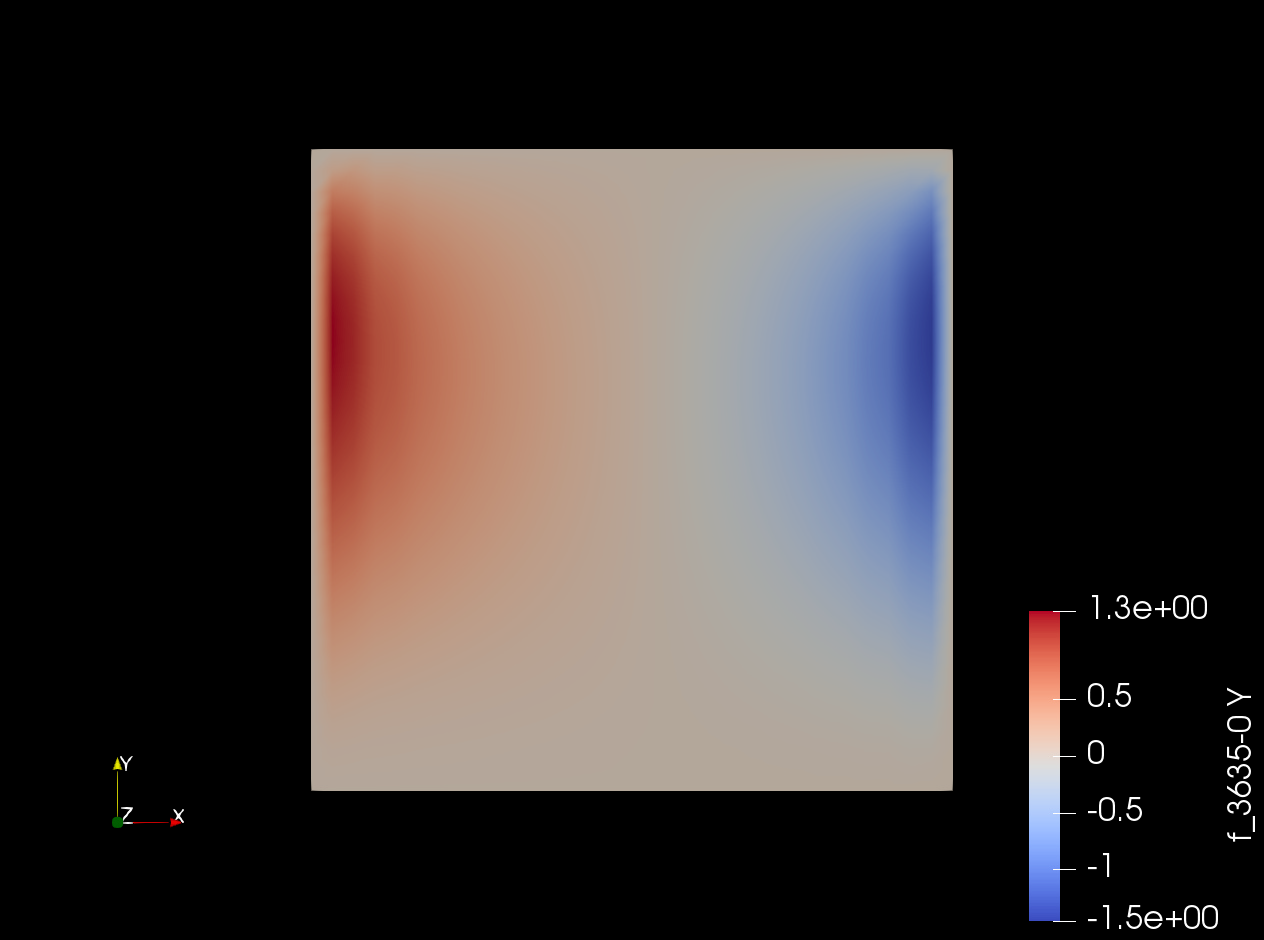
\includegraphics[width=0.9\linewidth]{../visualise_convergence_result/thesis_fenics_code_and_results/reference_folder/velocity_eps_conv/velocity_v_anis_1_19e-07}
  \captionof{figure}{$\textcolor{jasper}{\epsilon} = \mathcal{O}(-7).$}
\end{minipage}%
\begin{minipage}{0.35\textwidth}
  \centering
  
\includegraphics[width=0.9\linewidth]{../visualise_convergence_result/thesis_fenics_code_and_results/reference_folder/velocity_hydr/velocity_v_hydr}
  \captionof{figure}{$\textcolor{jasper}{\epsilon} = 0.0.$}
\end{minipage}

\end{figure}

\end{frame}

\begin{frame}{The perceived trend of the concentration solution}
\begin{figure}[H]
\centering
\begin{minipage}{0.35\textwidth}
  \centering
  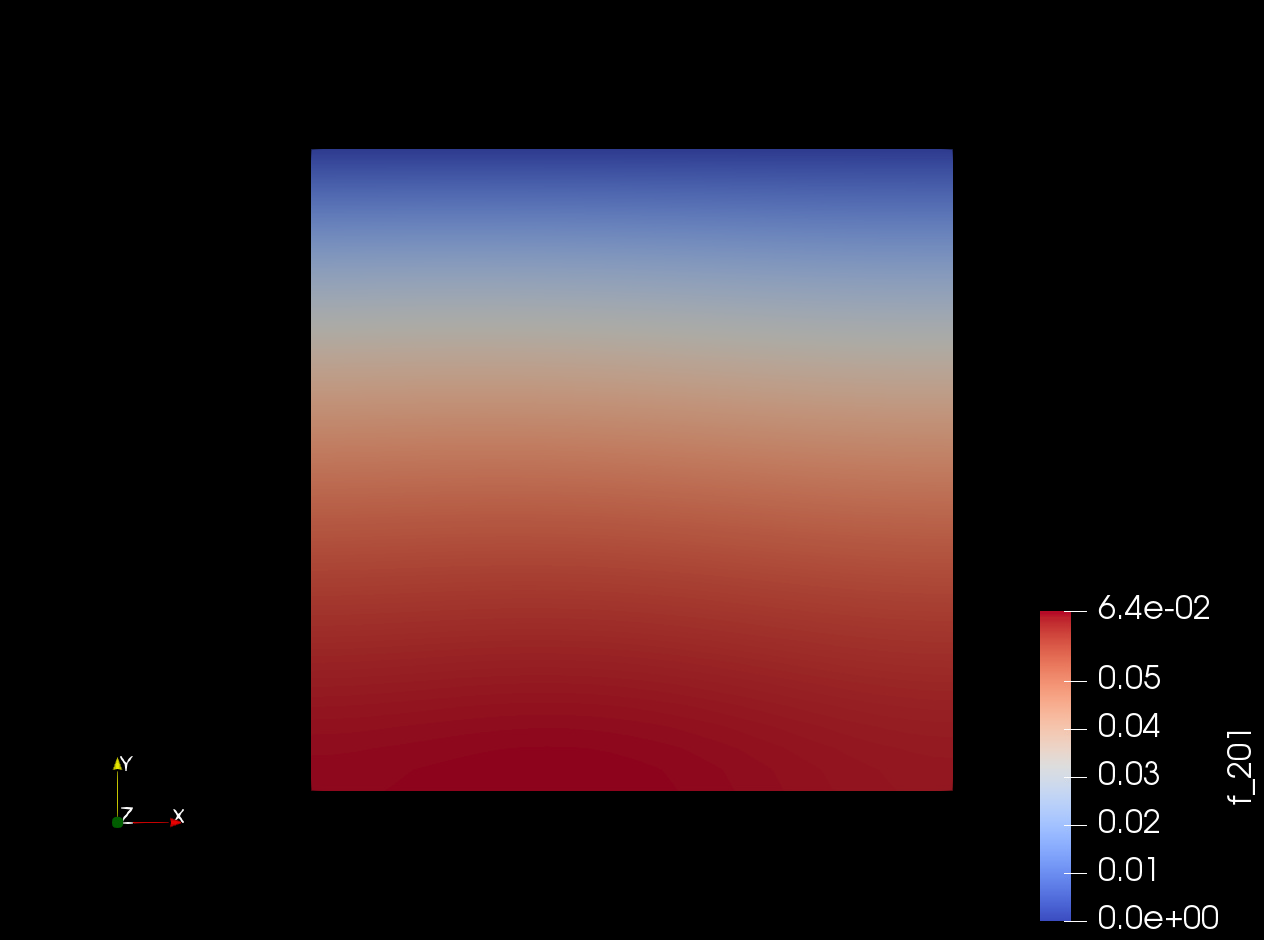
\includegraphics[width=0.9\linewidth]{../visualise_convergence_result/thesis_fenics_code_and_results/reference_folder/concentration_eps_conv/concentration_anis_1_00000}
  \captionof{figure}{$\textcolor{jasper}{\epsilon} = 1.0000000.$}
\end{minipage}%
\begin{minipage}{0.35\textwidth}
  \centering
  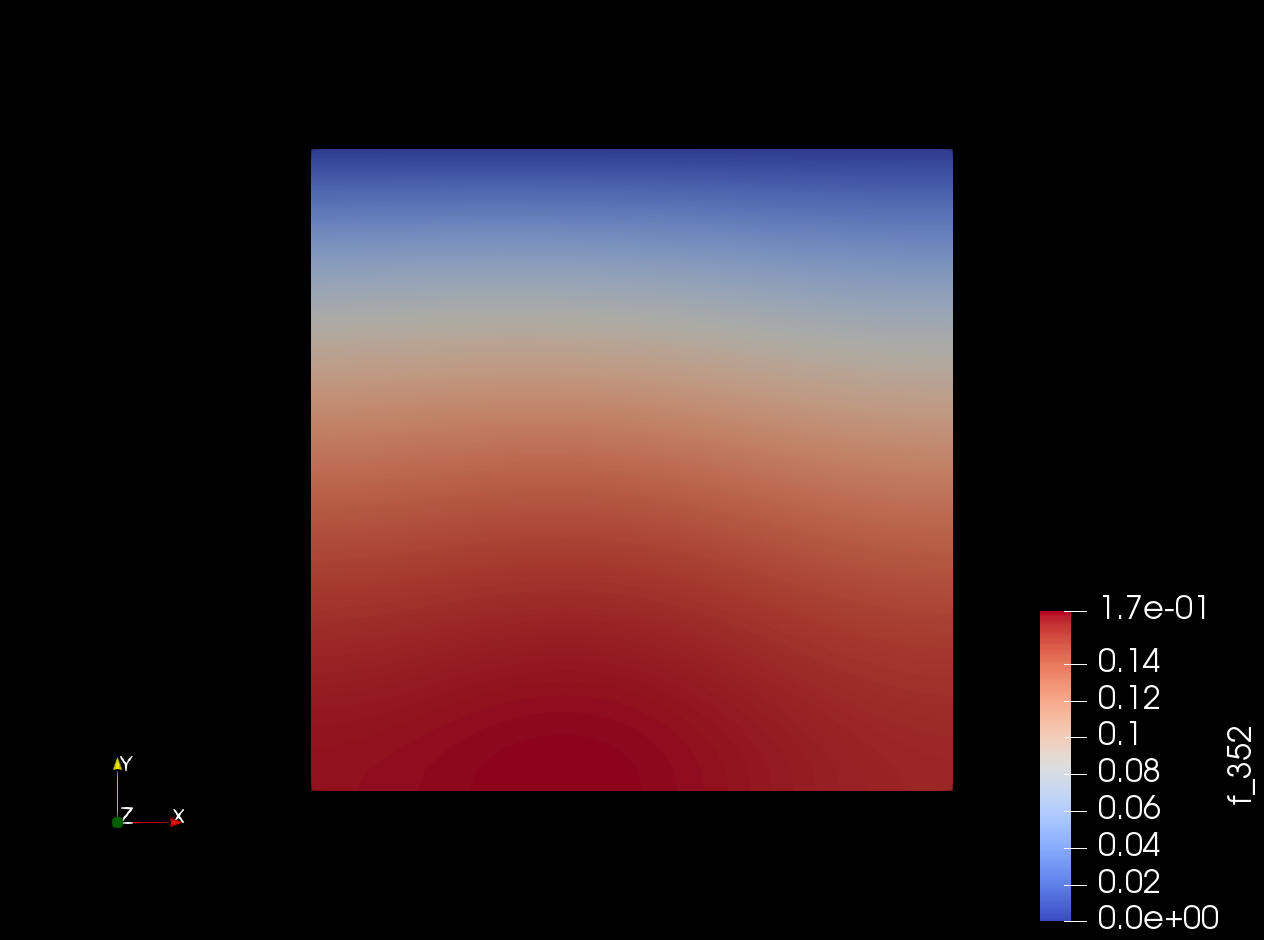
\includegraphics[width=0.9\linewidth]{../visualise_convergence_result/thesis_fenics_code_and_results/reference_folder/concentration_eps_conv/concentration_anis_0_50000}
  \captionof{figure}{$\textcolor{jasper}{\epsilon} = 0.5000000.$}
\end{minipage}
\end{figure}

\begin{figure}[H]
\centering
\begin{minipage}{0.35\textwidth}
  \centering
  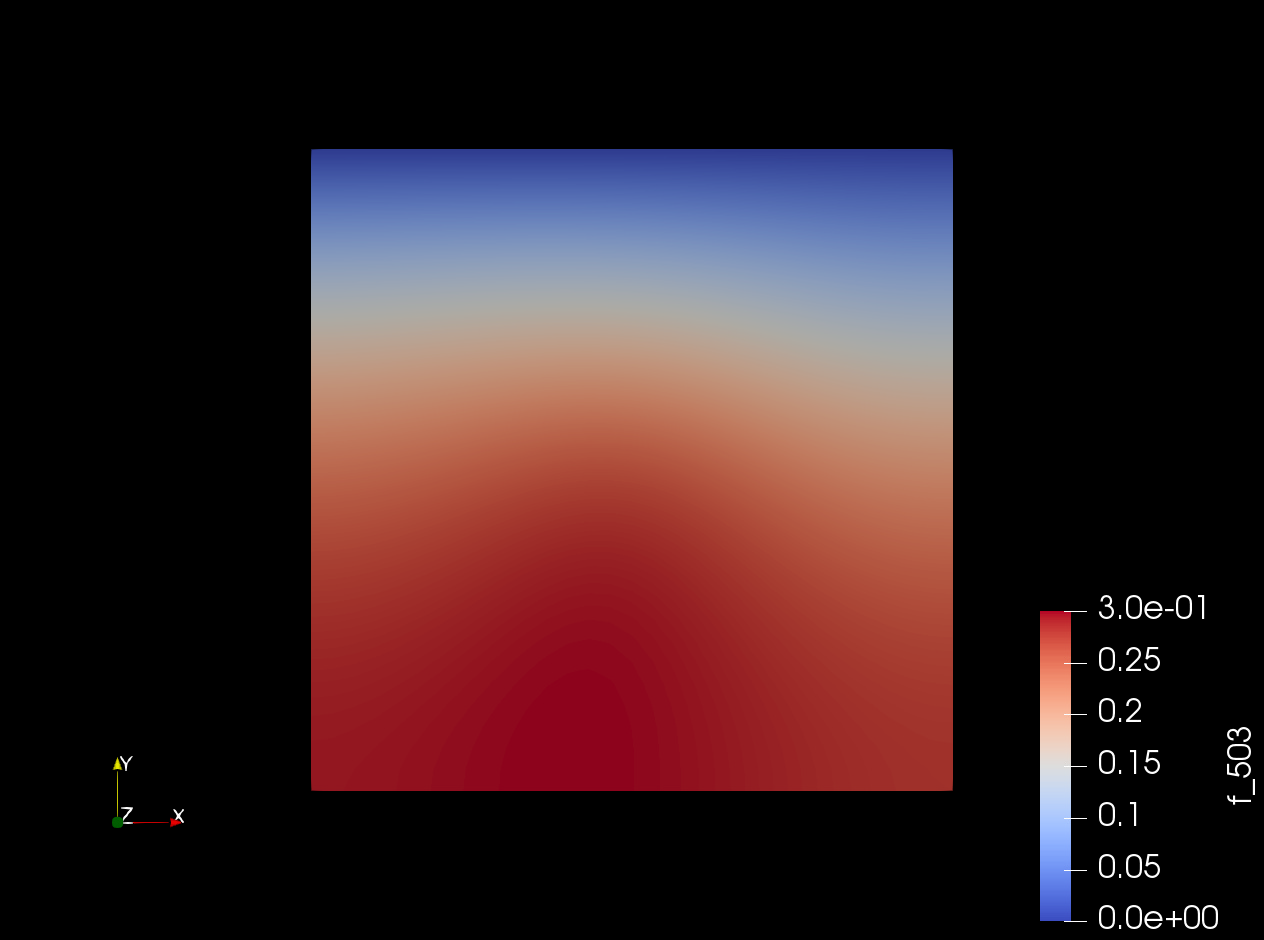
\includegraphics[width=0.9\linewidth]{../visualise_convergence_result/thesis_fenics_code_and_results/reference_folder/concentration_eps_conv/concentration_anis_0_25000}
  \captionof{figure}{$\textcolor{jasper}{\epsilon} = 0.2500000.$}
\end{minipage}%
\begin{minipage}{0.35\textwidth}
  \centering
  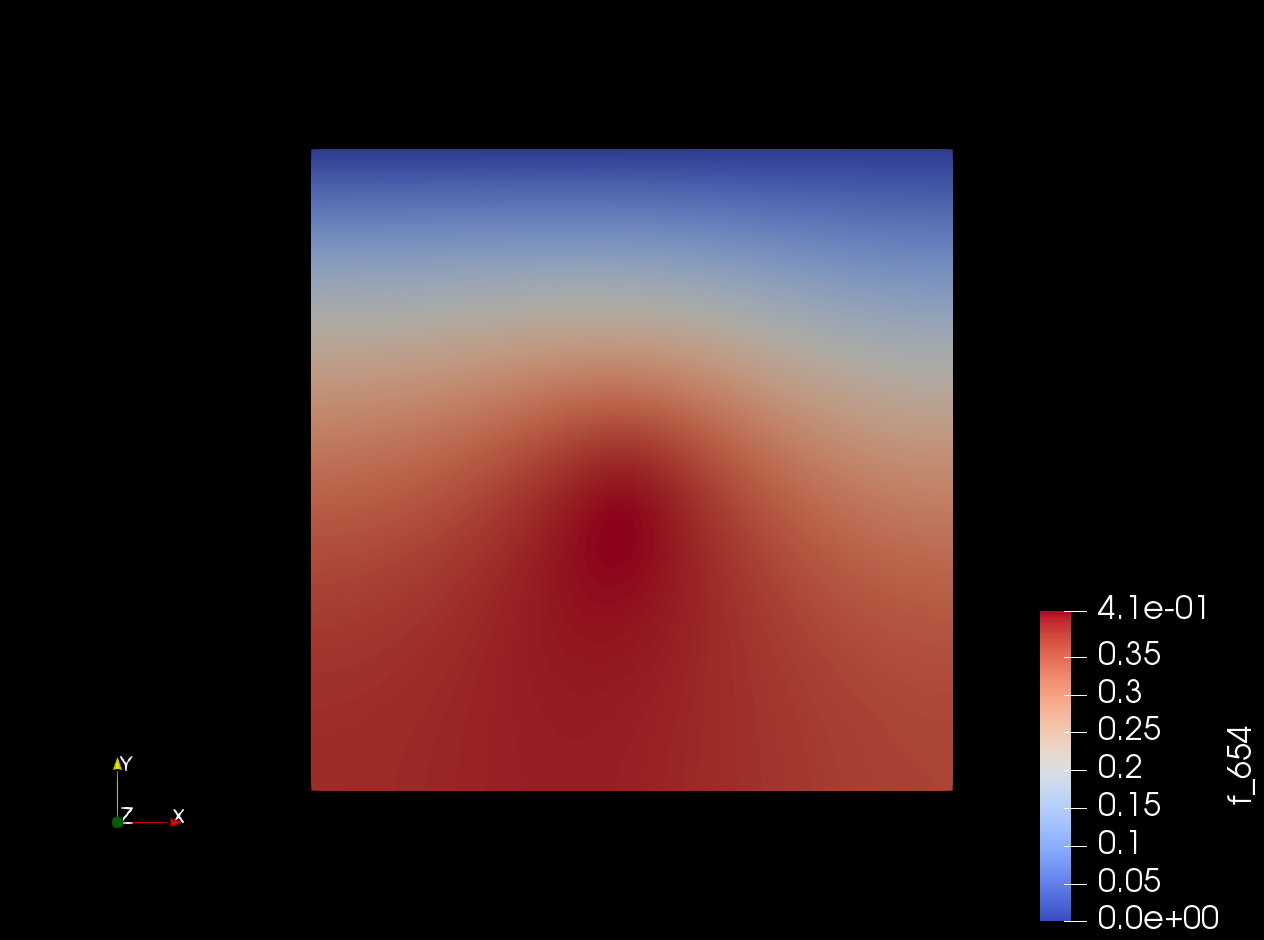
\includegraphics[width=0.9\linewidth]{../visualise_convergence_result/thesis_fenics_code_and_results/reference_folder/concentration_eps_conv/concentration_anis_0_12500}
  \captionof{figure}{$\textcolor{jasper}{\epsilon} = 0.1250000.$}
\end{minipage}
\end{figure}
\end{frame}

\begin{frame}

\begin{figure}[H]
\centering
\begin{minipage}{0.35\textwidth}
  \centering
  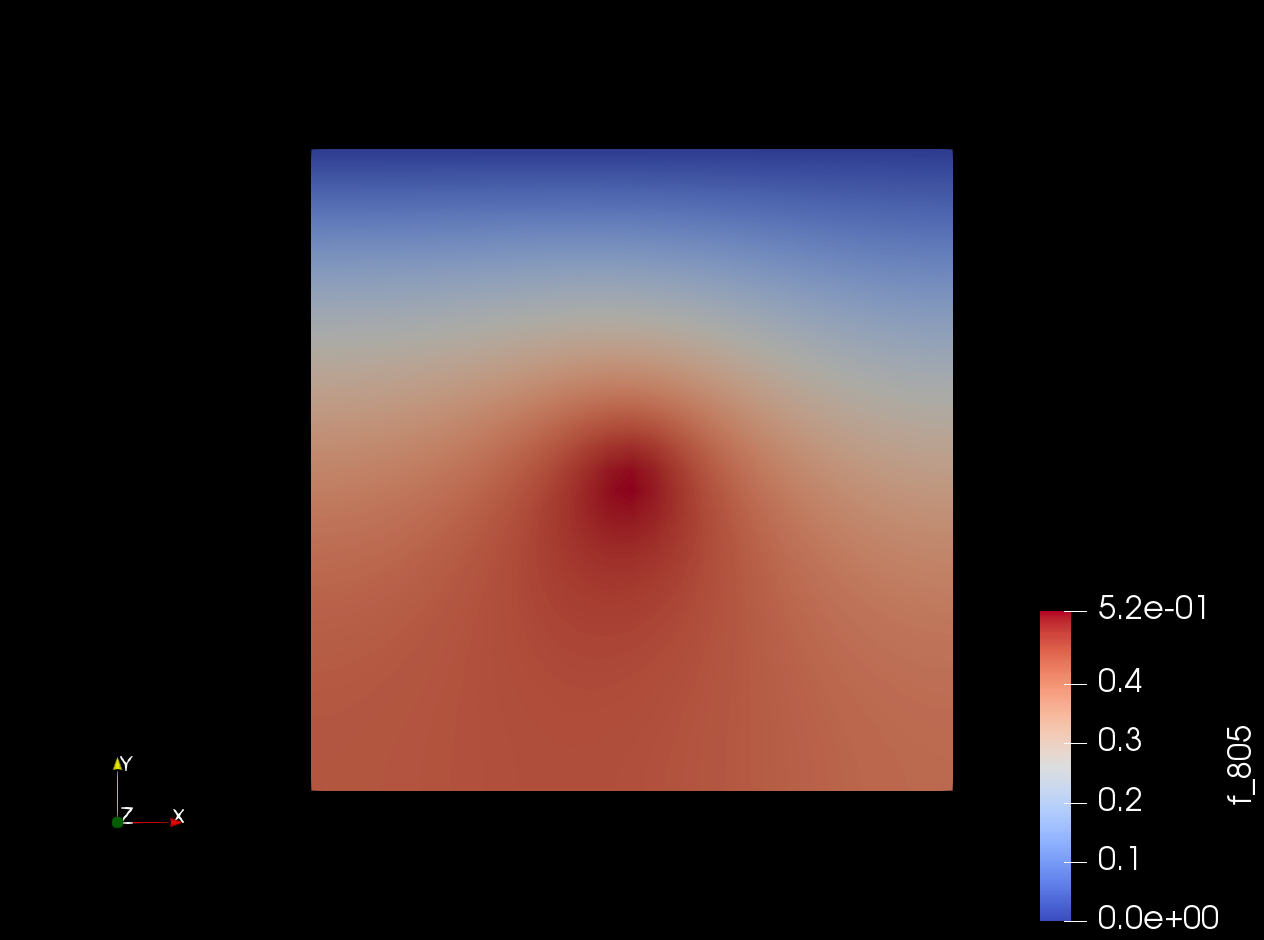
\includegraphics[width=0.9\linewidth]{../visualise_convergence_result/thesis_fenics_code_and_results/reference_folder/concentration_eps_conv/concentration_anis_0_06250}
  \captionof{figure}{$\textcolor{jasper}{\epsilon} = 0.0625000.$}
\end{minipage}%
\begin{minipage}{0.35\textwidth}
  \centering
  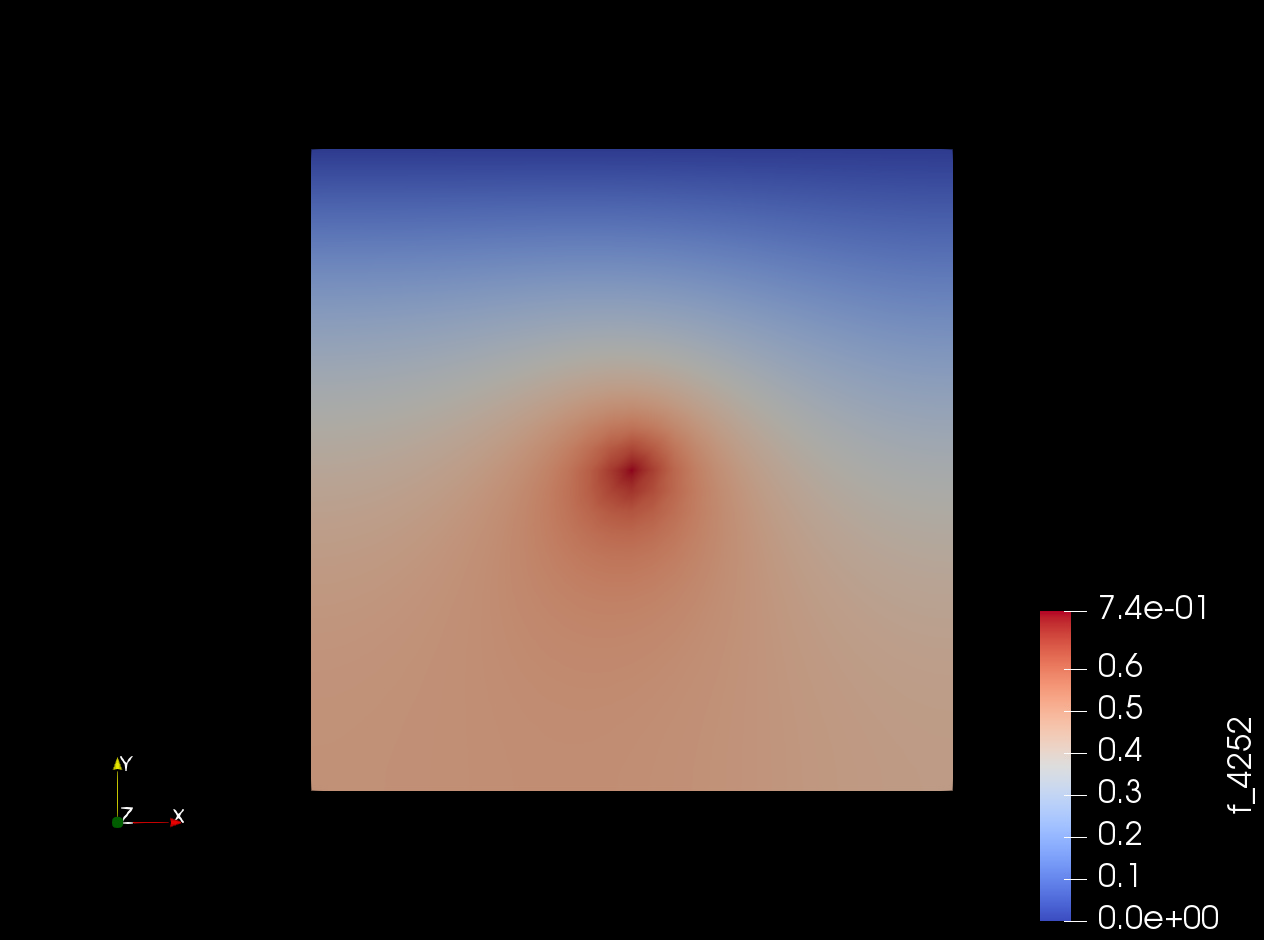
\includegraphics[width=0.9\linewidth]{../visualise_convergence_result/thesis_fenics_code_and_results/reference_folder/concentration_eps_conv/concentration_anis_0_01562}
  \captionof{figure}{$\textcolor{jasper}{\epsilon} = 0.015625.$}
\end{minipage}
\end{figure}

\begin{figure}[H]
\centering
\begin{minipage}{0.35\textwidth}
  \centering
  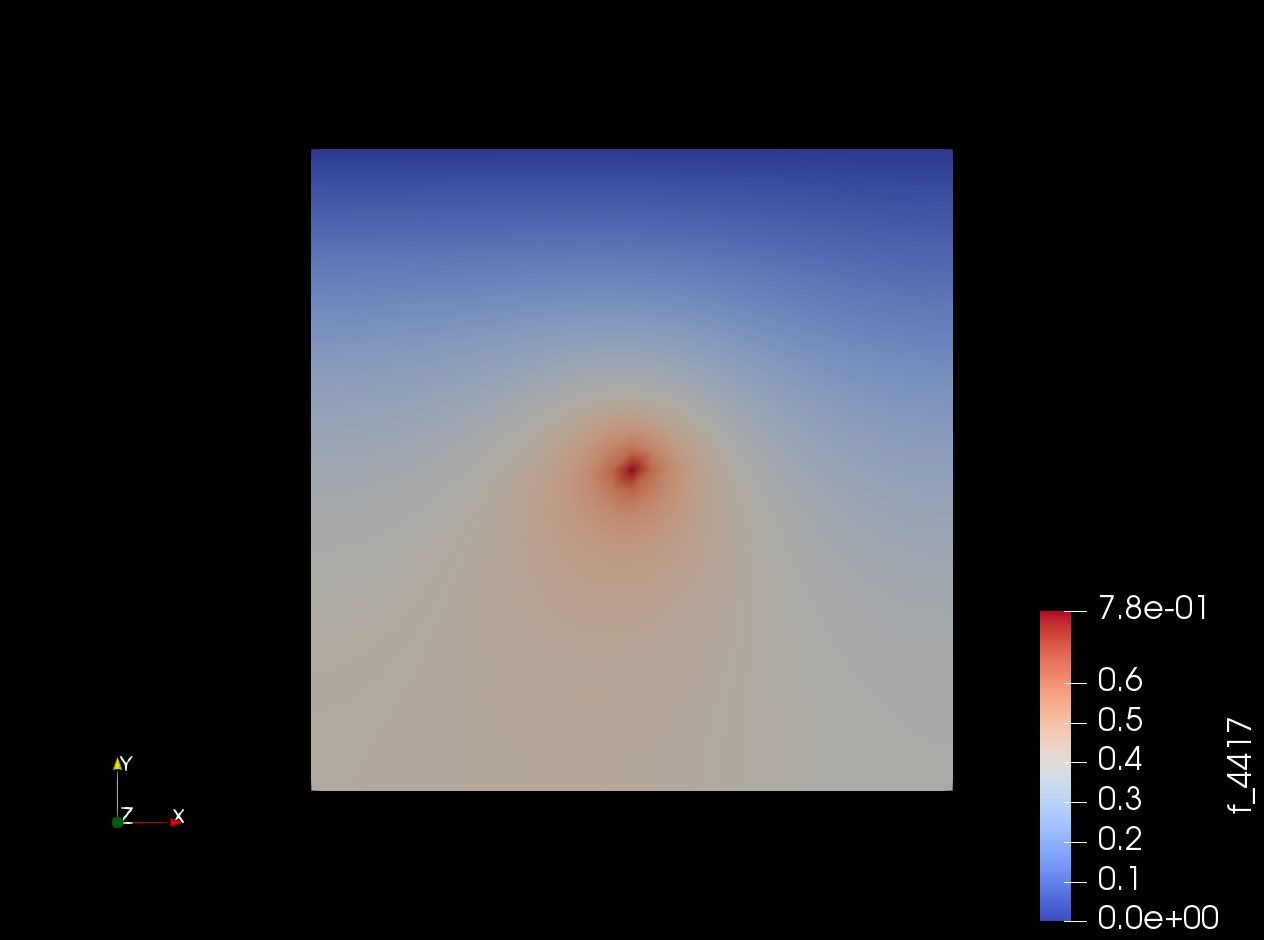
\includegraphics[width=0.9\linewidth]{../visualise_convergence_result/thesis_fenics_code_and_results/reference_folder/concentration_eps_conv/concentration_anis_0_00195}
  \captionof{figure}{$\textcolor{jasper}{\epsilon} = 0.00195.$}
\end{minipage}%
\begin{minipage}{0.35\textwidth}
  \centering
  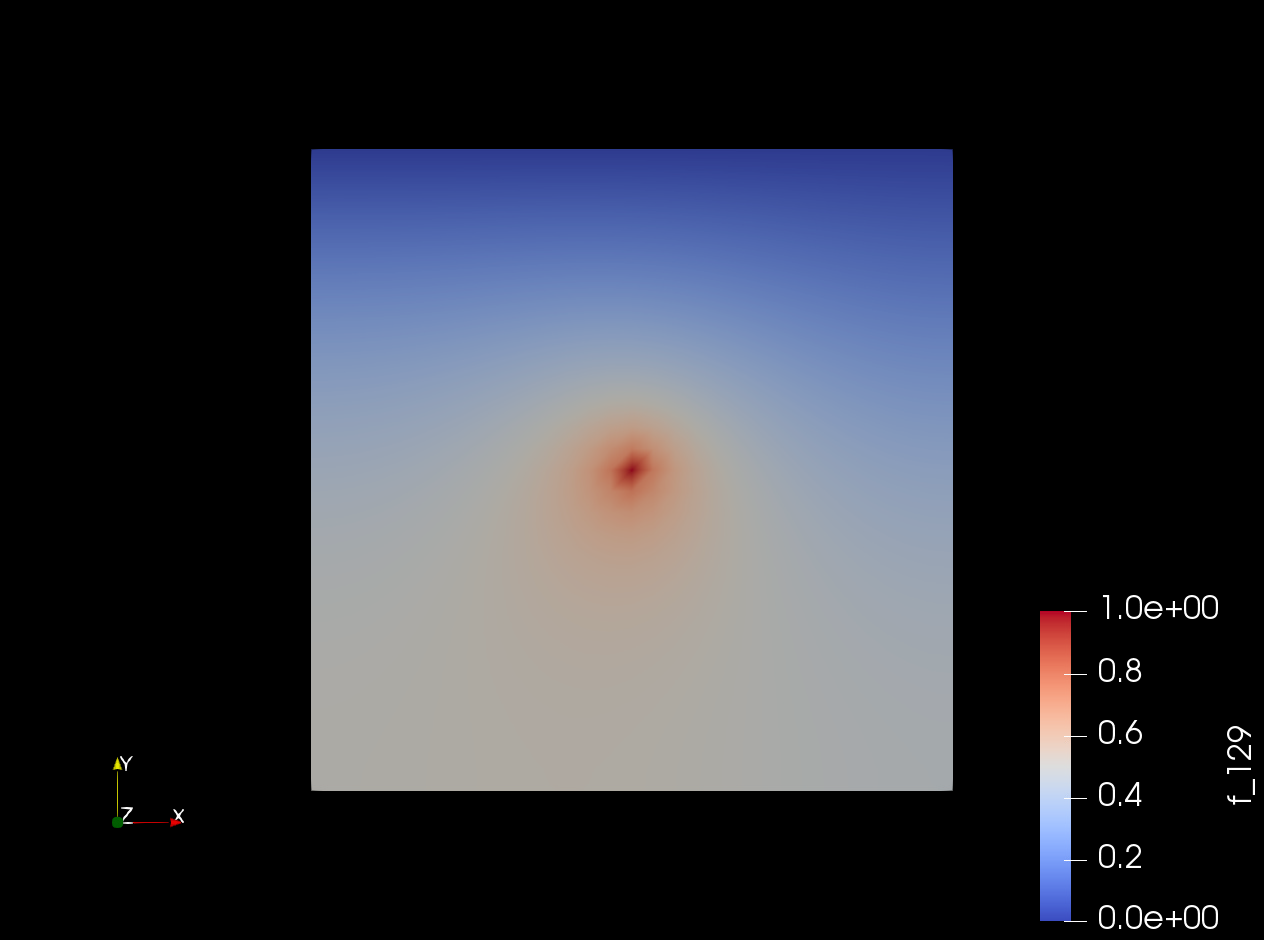
\includegraphics[width=0.9\linewidth]{../visualise_convergence_result/thesis_fenics_code_and_results/reference_folder/concentration_hydr/concentration_hydr}
  \captionof{figure}{$\textcolor{jasper}{\epsilon} = 0.0.$}
\end{minipage}
\end{figure}

\end{frame}

\end{document}